\section{Neural Networks}

\subsection{Deep Learning}

The concepts of deep learning studied in this section is going to be based on the work of \citet{goodfellow2016} and the documentation of PyTorch\footnote{\url{https://pytorch.org/docs/stable/index.html}} and MATLAB\footnote{\url{https://www.mathworks.com/help/matlab/}}.

There are several definitions of \gls*{ai} \citep{winston1992}, but the  computer scientist \citet{mccarthy2007} defines it as ``the science and engineering of making intelligent machines, especially intelligent computer programs.''.
He also states that ``it is related to the similar task of using computers to understand human intelligence, but AI does not have to confine itself to methods that are biologically observable.''.

The big area of study is the \gls*{ai} and it includes several branches like fuzzy logics, robotics, machine learning and so on. 
The later one, in turn, is another field with also some branches and one of them is the deep learning.
This can be represented in a Venn diagram, as the \cref{fig:venn_dl} shows.
However, all the three terms can be interchangeable in the major context.
%
\begin{figure}[!htb]
    \centering
    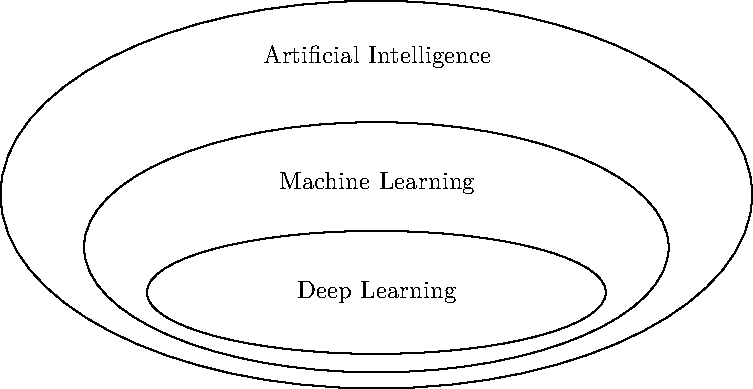
\includegraphics{figures/3review/nn/venn_dl.pdf}
    \caption{Subareas of Artificial Intelligence}
    \label{fig:venn_dl}
\end{figure}

The deep learning history goes back to the 1940s and it had several names over the years. 
It was called by \emph{cybernetics} (1940s--1960s), \emph{connectionism} (1980s--1990s), and from 2006 until now is known as \emph{deep learning}.
The \gls*{dl} models were engineered systems inspired by the biological brain and they were denominated \gls*{ann}.
One of the motivations of the neural  perspective was to understand that the brain provides a proof by example that intelligent behavior is possible and try to reverse engineer the computation principals behind the brain, duplicating its functionality.
Today it goes beyond the neuroscientist perspective and it is more of general principle of learning multiple levels of composition.

\gls*{dl} dwells in the programming sphere. The approach, however, it is not like the traditional programming scripts and models. To automate stuff, there are three main parts: (i) the input data, (ii) the rule (function) and (iii) the output data. In both types there are two of three parts available, but different ones for each other. In the traditional programming, there is the input data and the rule, for the algorithm output the data. In deep learning, there is the input data and the output data, for the algorithm provides the rule. A good analogy is cooking: in the traditional programming context, one has the ingredients and the recipe to make the main course; in the deep learning context, one has the ingredients and the main course to discover the recipe.

\subsection{Neural Networks Models}

\subsection{Loss Function}

The \emph{loss function}, also called \emph{cost function} or \emph{error function}, is the one used measure the error between the predicted output of an algorithm and the real target output. 
There are several loss functions suitable to different kind of situation. For each distributed data there is one that fits better.
%
\begin{figure}[!htb]
    \centering
    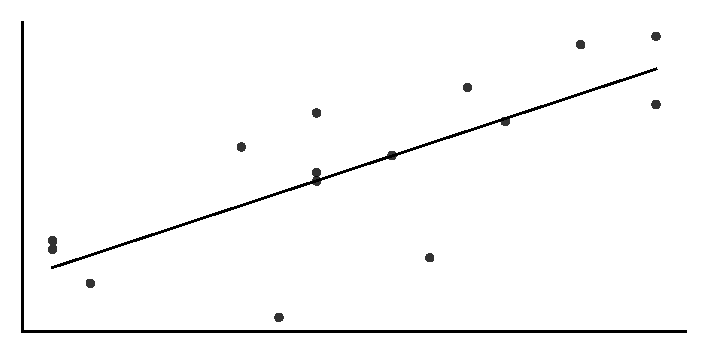
\includegraphics{figures/3review/nn/mae_chart.pdf}
    \caption[Linear Data and Loss Function]{Linear Data and Loss Function. The loss function take all the distances between the predicted and the target value to verify if the model is in the right path. The lower the distance, the better.}
    \label{fig:mae_chart}
\end{figure}

For a linear distribution of the data, for instance, a common loss function adopted is the \gls*{mse} \citep{bussab2017} or \gls*{mae}.
%
\begin{align}
    \mse &= \frac{1}{n} \sum_{i=1}^n (y_i - x_i)^2
    \label{eq:mse} \\
    \mae &= \frac{1}{n} \sum_{i=1}^n |y_i - x_i|
    \label{eq:mae}
\end{align}
%
where \(n\) is the sample size; \(y_i\) is the predicted output; and \(x_i\) is the real target.

\gls*{mae} and \gls*{mse} are simple methods and both lead to poor results for complex data patterns.
Although, through them, it is easy to recognize the essence of what the cost function does. 
Other methods like \emph{cross-entropy} are more likely to get better results when having a pattern of complex data.

Therefore, the loss function measures how far from the real value the data is. Many kinds of them are available and must be analyzed the most proper one to each case. 
It will depend on not only the data and its pattern, but also the computational processing and the cost attached to it.

\subsubsection*{Cross Entropy}

\subsubsection*{Binary Cross Entropy}

\subsection{Optimizer}

The optimizer is an algorithm that updates the model in response to the output of the loss function, that is, it aids to minimize the loss function. 
As the loss function minimizes, the model is getting closer to the target values and, hence, closer to the real pattern.

The \emph{gradient descent} is one of the main algorithm \citep{nesterov2004} that optimizes the model and many important ones are based on it, like the \gls*{sgd}. The goal is to get the minimum, as the error (loss) between the predicted and the target data is null. This would mean that the model fits to the pattern of the data.
%
\begin{figure}[!htb]
    \centering
    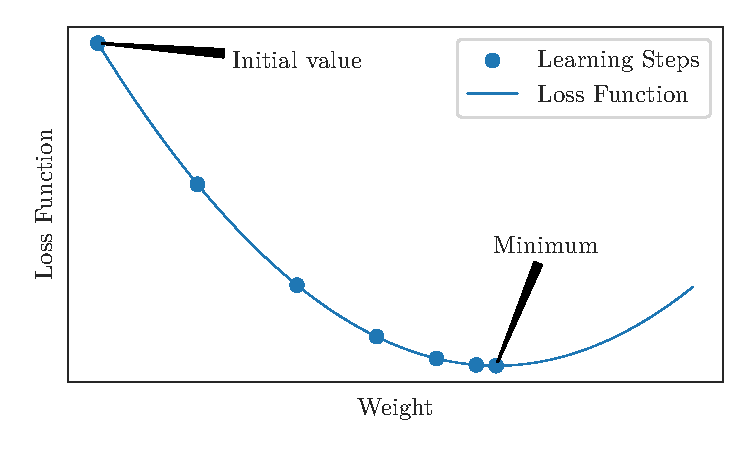
\includegraphics{figures/3review/nn/gradient_descent.pdf}
    \caption[Gradient Descent Process]{Gradient Descent Process. In this case, the loss function can be represented in a two-axes plan. Depending on the data, it is not possible to represent graphically due to its multi dimension.}
\end{figure}

\subsubsection*{Gradient Descent} 

The gradient descent is a powerful algorithm that reduces the loss function, minimizing the error between the predicted value and the target value.

Since the gradient of a function gives the direction of the steepest ascent of a function and it is orthogonal to the surface at a determined point, it seems reasonable that moving in the perpendicular direction gives the maximum increase of the function \cite{stewart2016}.
On the other hand, the negative of the gradient may be used to find the opposite, that is, the steepest descent of the function, or the minimum decrease.
If the steps given to the direction of the negative gradient of the function are small, there is a good chance to get minimum value of the function.
However, if the steps are too long, the chance to pass by the minimum value is high \citep{nielsen2015}.
These steps are called \emph{learning rate} and should be chosen wisely.

This way, let \(\symbf{x}\) be the entry vector with the predicted data and \(L\) the loss function adopted for some deep learning model, and \(\epsilon\) the learning rate, the gradient descent is:
%
\begin{equation}
    \symbf{x}_{t+1} = \symbf{x}_t - \epsilon \nabla L(\symbf{x}_t)
\end{equation}

In determined cases, it is possible to avoid running the iterative algorithm and just go directly to the critical point by solving \(\nabla L(\symbf{x}_t) = 0\) for \(\symbf{x}\).

\subsubsection*{Stochastic Gradient Descent}

As seen, gradient descent is a powerful tool to minimize the loss function, however, for large data, the cost of operation is very high and its use is not feasible. 
The main ideia of \gls*{sgd} is that the gradient is an expectation.
Later, the data is divided in subsets, also called \emph{mini-batch} and then the gradient is performed over them.
The mini-batche size is chosen to be a realatively small numbers of examples.
The data inside each subset may be considered redundant, that is why it uses one single value of the subset to compute the gradient descent.
This way, the process is considerable better for computational resources.

The \gls*{sgd} can be written as:
%
\begin{equation}
    \symbf{x}_{t+1} = \symbf{x}_t - \frac{\epsilon}{m} \sum_{i=1}^m \nabla L(\symbf{x}_t; p^{(i)},q^{(i)})
\end{equation}
%
where \(m\) is the mini-batch size, and \(\nabla L(\symbf{x}; p^{(i)}, q^{(i)})\) is the gradient of the loss function with respect to the parameter vector \(\symbf{x}\) for the \(i^{\text{th}}\) example \((p^{(i)}, q^{(i)})\) in the mini-batch.

Yet, nowadays, with the amount of data, many techniques are still applied in \gls*{sgd} as creating an automatic adaptive learning rates which achieve the optimal rate of convergence \citep{darken1991} and the momentum technique to improve it \citep{sutskever2013}.